\subsection{Handling ``fast'' cards}
	
For very simple cards (e.g. words in different language that are so similar), it
might be a bit annoying to have to answer these cards again and again in every
partition.  Such \emph{fast} cards can be marked as such and handled
differently:  If a fast card is gotten right once it should be immediately moved
to the last partition in the box.  This way the card is learnt once and is
tested only once more before it is finally removed from the box.

To introduce fast cards to our learning box go to the metamodel and create a new
eclass \texttt{FastCard}.  Quick link to \texttt{Card} and choose
\texttt{Inheritance} from the quick link context menu
(Fig.~\ref{fig:sdm_fastcard_1}). 

\begin{figure}[htp]
\begin{center}
  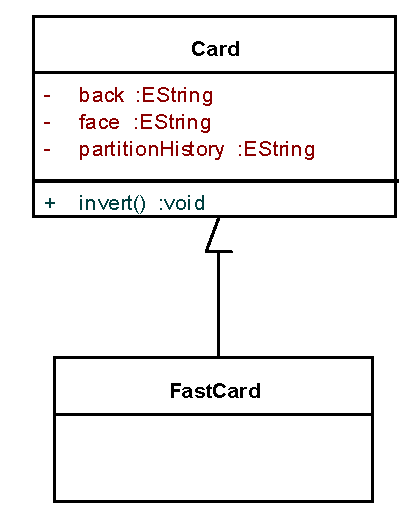
\includegraphics[width=0.35\textwidth]{pics/sdmBilder/bindings/fastcard}
  \caption{Fast cards are a special kind of card.}  
  \label{fig:sdm_fastcard_1}
\end{center}
\end{figure}

Now go to the SDM \texttt{check} in \texttt{Partition} and extend the control
flow as depicted in Fig.~\ref{fig:sdm_fastcard_2}.  Add new story nodes
\texttt{is fast card?} and \texttt{promote fast card} and drag and drop a bound
object variable \texttt{fastcard} \emph{of type} \texttt{FastCard} into
\texttt{is fast card?}.  What we need to do now is decide, based on the dynamic
type\footnote{In a statically typed language like Java, every object has a
static type (determined at compile time) and a dynamic type (that can only be
determined at runtime).} of \texttt{card} if we must handle a fast card or not.

This can be expressed in SDMs via \emph{BindingExpressions} or just
\emph{Bindings}.  A binding can be specified for a \emph{bound} object variable
\note{Bindings}
and represents the final case where an object variable can be marked as being
bound.  

To refresh your memory, we have already learnt that a bound object
variable is either (1) assigned to \texttt{this}, (2) a parameter of the method,
or (3) a value determined in a preceding activity node.  Bindings represent a
fourth possibility of giving a manual binding for an object variable. 

\begin{figure}[htbp]
\begin{center}
  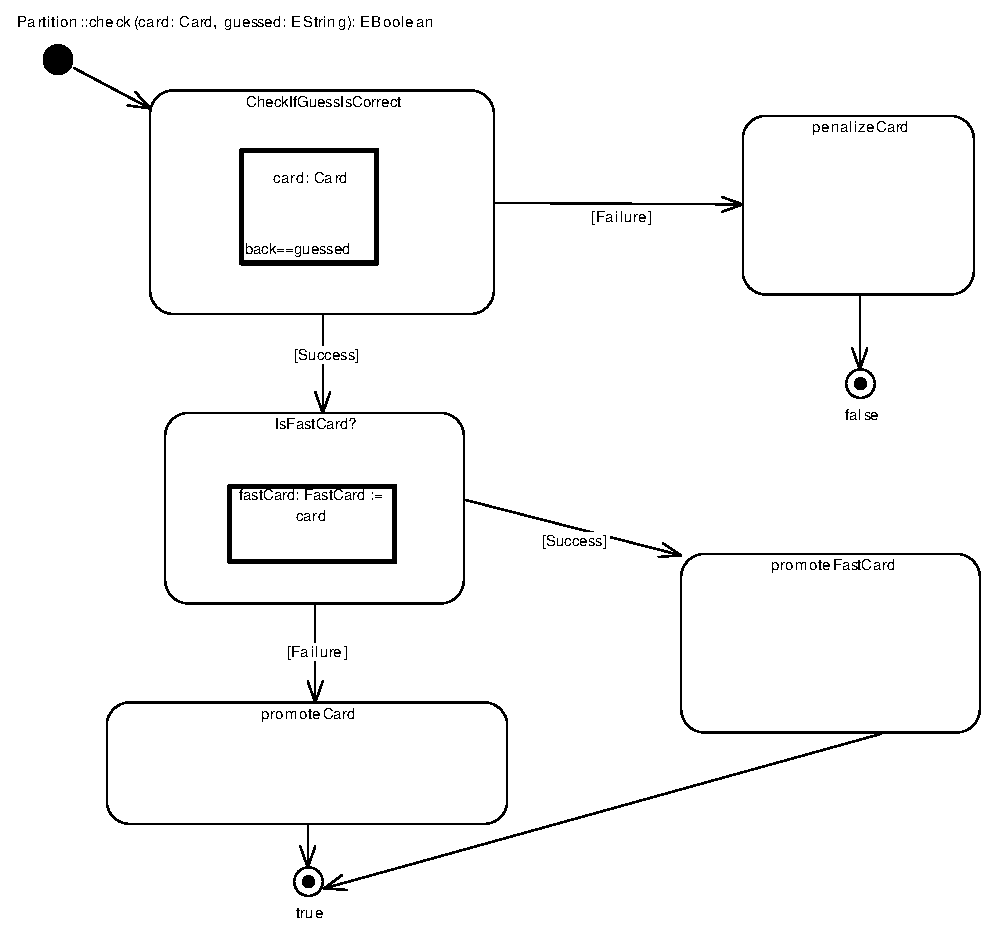
\includegraphics[width=0.6\textwidth]{pics/sdmBilder/bindings/fastcard_controlflow}
  \caption{Extend check to handle fast cards.}  
  \label{fig:sdm_fastcard_2}
\end{center}
\end{figure}

To create a binding for \texttt{fastcard}, choose the \texttt{Binding} tab in
the \texttt{Object Variable Properties} dialogue
(Fig.~\ref{fig:sdm_fastcard_3}). 

\begin{figure}[htbp]
\begin{center}
  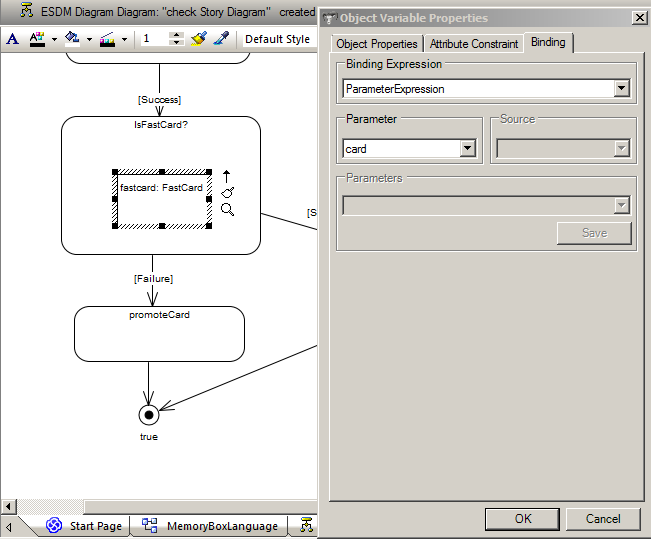
\includegraphics[width=0.427\textwidth]{pics/sdmBilder/bindings/fastcard_bindingexp.png}
  \caption{Create a binding for \texttt{fastcard}.}  
  \label{fig:sdm_fastcard_3}
\end{center}
\end{figure}

\clearpage

As usual all our expression types can be used for the \texttt{Binding
Expression}.  Since we already know all the types let's consider what each type
would mean in this context: 
\begin{description}
  \item[MethodCallExpression:]~\\ This would allow invoking a method and binding
  its return value to the object variable.  This is how non-primitive return
  values of methods can be used safely in SDMs.
  \item[ParameterExpression:]~\\ This could be used to bind the object variable
  to a parameter of the method.  If the object variable is of a different type
  than the parameter (e.g. a subtype) this represents basically a successful
  typecast if the pattern matches.
  \item[LiteralExpression:]~\\ As usual this can be anything and is literally
  copied with a surrounding typecast into the generated code.  Using
  LiteralExpressions too often is usually a sign for not thinking in a
  \emph{pattern oriented} manner and is considered a \emph{bad smell}.
  \item[ObjectVariableExpression:]~\\ This can be used to refer to other object
  variables in preceding story nodes.  Just like for ParameterExpressions, this
  represents a simple typecast if the types of the \texttt{target} and the
  object variable with the binding are different.
\end{description}

In our case, we could use a ParameterExpression or an ObjectVariableExpression as
\texttt{card} is indeed a parameter \emph{and} has already been used in
\texttt{checkIfGuessIsCorrect}.  As we haven't used ObjectVariableExpressions
before lets try it out!  Choose \texttt{ObjectVariableExpression} as the type of
the binding expression and \texttt{card} from the drop-down menu as the target. 
If you've done everything right, the binding should be visualised concisely as
in Fig.~\ref{fig:sdm_fastcard_4}.
 
\begin{figure}[htbp]
\begin{center}
  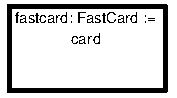
\includegraphics[width=0.3\textwidth]{pics/sdmBilder/bindings/visual_bindingexp}
  \caption{Visualisation for binding expression.}  
  \label{fig:sdm_fastcard_4}
\end{center}
\end{figure}

\clearpage

To complete the SDM, extract the story pattern of \texttt{promote fast card} and
specify the pattern according to Fig.~\ref{fig:sdm_fastcard_5}.  The fast card
is transferred from the current partition \texttt{this}, to the last partition
in the box, which is identified with an appropriate \mbox{NAC} (already used in
Sec.~\ref{sec:sdm_grow}). 

\begin{figure}[htbp]
\begin{center}
  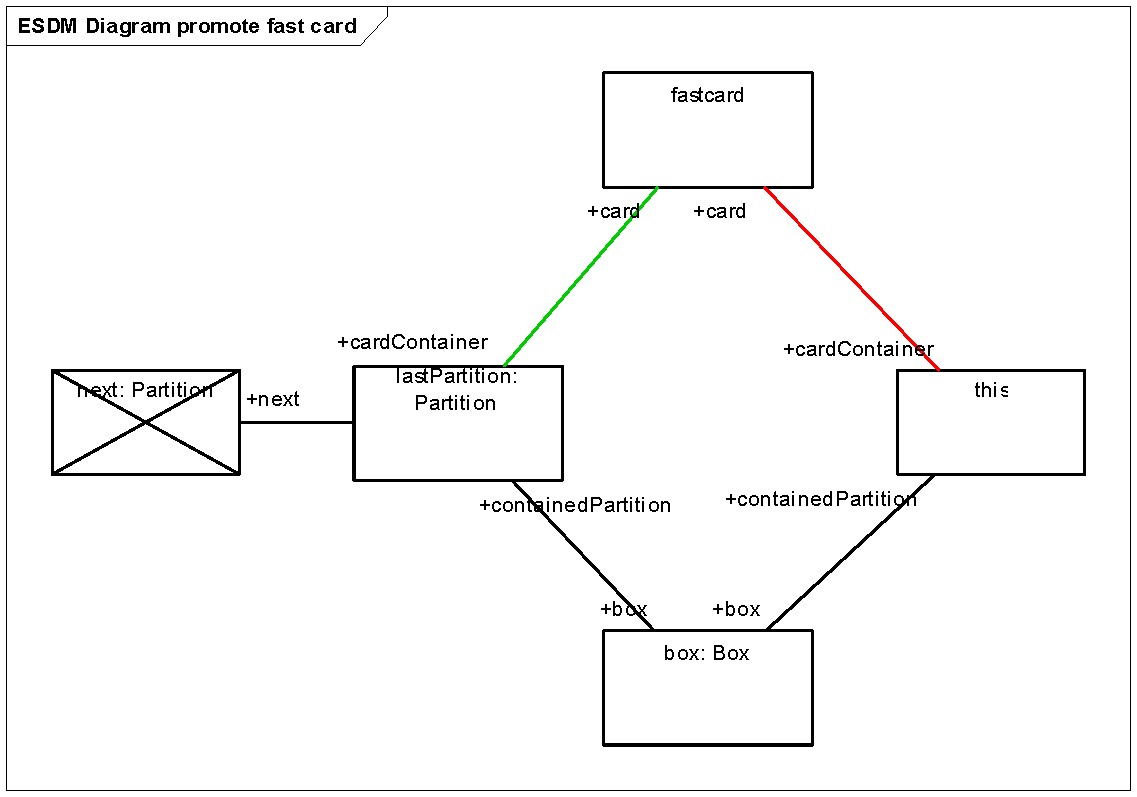
\includegraphics[width=0.8\textwidth]{pics/sdmBilder/bindings/promoteFastCard}
  \caption{Story pattern for handling fast cards.}  
  \label{fig:sdm_fastcard_5}
\end{center}
\end{figure}

Export, generate code and inspect the new implementation for \texttt{check}. 
Can you find the generated type casts for \texttt{fastcard}?  Don't forget to
write a few tests and see if fast cards are handled correctly!


